%
% riemann.tex
%
% (c) 2020 Prof Dr Andreas Müller, Hochschule Rapperswil
%
\begin{frame}[fragile]
\frametitle{Riemann-Integral}
\vspace{-20pt}
\begin{columns}[t]
\begin{column}{0.40\hsize}
\uncover<2->{%
\begin{block}{Unterteilung}
\vspace{-20pt}
\[
a=x_0 < x_1 < \dots < x_{n-1} < x_n = b
\]
\end{block}}
\vspace{-10pt}
\uncover<3->{%
\begin{block}{Maximal- und Minimalwerte}
\vspace{-20pt}
\begin{align*}
\overline{f}_k
&=\max\{
f(x)\;|\;
x\in[x_{k-1},x_k]
\}
\\
\underline{f}_k
&=
\min\{
f(x)\;|\;
x\in[x_{k-1},x_k]
\}
\end{align*}
\end{block}}
\vspace{-10pt}
\uncover<4->{%
\begin{block}{Ober- und Untersummen}
\vspace{-15pt}
\begin{align*}
\underline{I}
&=
\sum_{k=1}^n \underline{f}_k (x_k-x_{k-1})
\\
\overline{I}
&=
\sum_{k=1}^n \overline{f}_k (x_k-x_{k-1})
\end{align*}
\end{block}}
\end{column}
\begin{column}{0.56\hsize}
\vspace{-10pt}
\begin{center}
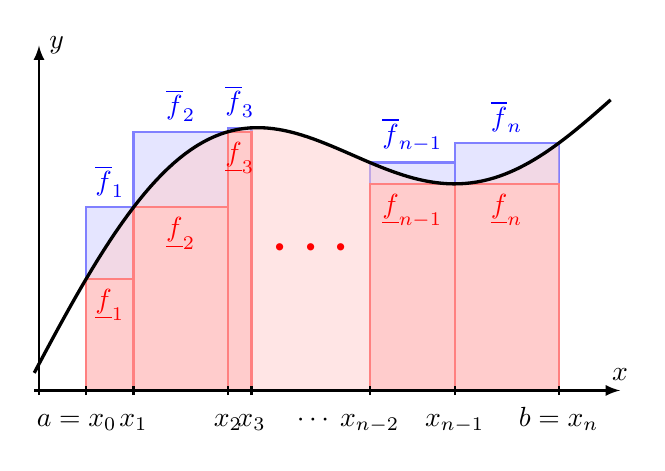
\begin{tikzpicture}[>=latex,thick,scale=0.6]

\def\A{2}
\def\B{0.5}
\def\C{0.04}
\def\D{1.8}

\def\a{1}
\def\xone{2}
\def\xtwo{4}
\def\xthree{4.5}
\def\xminustwo{7}
\def\xminus{8.8}
\def\b{11}

\def\oberesrechteck#1#2#3#4{
	\uncover<3>{
	\draw[color=blue!50] (#2,#3)--(#1,#3);
	}
	\uncover<4->{
	\fill[color=blue!10] (#1,0)--(#2,0)--(#2,#3)--(#1,#3)--cycle;
	\draw[color=blue!50] (#1,0)--(#2,0)--(#2,#3)--(#1,#3)--cycle;
	}
	\uncover<3->{
	\node[color=blue] at ({0.5*(#1+#2)},{#3}) [above] {#4};
	}
}

\def\unteresrechteck#1#2#3#4{
	\uncover<3>{
	\draw[color=red!50] (#2,#3)--(#1,#3);
	}
	\uncover<4->{
	\fill[color=red!20] (#1,0)--(#2,0)--(#2,#3)--(#1,#3)--cycle;
	\draw[color=red!50] (#1,0)--(#2,0)--(#2,#3)--(#1,#3)--cycle;
	}
	\uncover<3->{
	\node[color=red] at ({0.5*(#1+#2)},{#3}) [below] {#4};
	}
}

\oberesrechteck{\a}{\xone}{{\A+\B*\xone-\C*(\xone-6)*(\xone-6)+\D*sin(90*\xone/3.14)}}{$\overline{f}_1$};
\oberesrechteck{\xone}{\xtwo}{{\A+\B*\xtwo-\C*(\xtwo-6)*(\xtwo-6)+\D*sin(90*\xtwo/3.14)}}{$\overline{f}_2$};
\oberesrechteck{\xtwo}{\xthree}{{\A+\B*\xthree-\C*(\xthree-6)*(\xthree-6)+\D*sin(90*\xthree/3.14)}}{$\overline{f}_3$};

\oberesrechteck{\xminustwo}{\xminus}{{\A+\B*\xminustwo-\C*(\xminustwo-6)*(\xminustwo-6)+\D*sin(90*\xminustwo/3.14)}}{$\overline{f}_{n-1}$};
\oberesrechteck{\xminus}{\b}{{\A+\B*\b-\C*(\b-6)*(\b-6)+\D*sin(90*\b/3.14)}}{$\overline{f}_n$};

\fill[color=red!20,opacity=0.5]
	plot[domain=1:11,samples=100]
		(\x,{\A+\B*\x-\C*(\x-6)*(\x-6)+\D*sin(90*\x/3.14)})
	-- (\b,0)--(\a,0)--cycle;

\unteresrechteck{\a}{\xone}{{\A+\B*\a-\C*(\a-6)*(\a-6)+\D*sin(90*\a/3.14)}}{$\underline{f}_1$}
\unteresrechteck{\xone}{\xtwo}{{\A+\B*\xone-\C*(\xone-6)*(\xone-6)+\D*sin(90*\xone/3.14)}}{$\underline{f}_2$}
\unteresrechteck{\xtwo}{\xthree}{{\A+\B*\xtwo-\C*(\xtwo-6)*(\xtwo-6)+\D*sin(90*\xtwo/3.14)}}{$\underline{f}_3$}

\unteresrechteck{\xminustwo}{\xminus}{{\A+\B*\xminus-\C*(\xminus-6)*(\xminus-6)+\D*sin(90*\xminus/3.14)}}{$\underline{f}_{n-1}$}
\unteresrechteck{\xminus}{\b}{{\A+\B*\xminus-\C*(\xminus-6)*(\xminus-6)+\D*sin(90*\xminus/3.14)}}{$\underline{f}_n$}

\draw[line width=1.2pt] plot[domain=-0.1:12.1,samples=100]
	(\x,{\A+\B*\x-\C*(\x-6)*(\x-6)+\D*sin(90*\x/3.14)});


% add image content here
\draw[->] (-0.1,0)--(12.3,0) coordinate[label={$x$}];
\draw[->] (0,-0.1)--(0,7.3) coordinate[label={right:$y$}];

\uncover<2->{%
\draw (\a,-0.1)--(\a,0.1); \node at ({\a-0.2},-0.1) [below] {$\mathstrut a=x_0$};
\draw (\b,-0.1)--(\b,0.1); \node at (\b,-0.1) [below] {$\mathstrut b=x_n$};

\draw (\xone,-0.1)--(\xone,0.1);
\node at (\xone,-0.1) [below] {$\mathstrut x_1$};

\draw (\xtwo,-0.1)--(\xtwo,0.1);
\node at (\xtwo,-0.1) [below] {$\mathstrut x_2$};

\draw (\xthree,-0.1)--(\xthree,0.1);
\node at (\xthree,-0.1) [below] {$\mathstrut x_3$};

\node at (5.75,-0.1) [below] {$\mathstrut\cdots$};
\node[color=red] at (5.75,3) {\Huge$\cdots$};

\draw (\xminustwo,-0.1)--(\xminustwo,0.1);
\node at (\xminustwo,-0.1) [below] {$\mathstrut x_{n-2}$};

\draw (\xminus,-0.1)--(\xminus,0.1);
\node at (\xminus,-0.1) [below] {$\mathstrut x_{n-1}$};
}

\end{tikzpicture}
\end{center}
\[
\uncover<5->{
\underline{I}
\le}
\int_a^b f(x)\,dx
\uncover<5->{
\le 
\overline{I}}
\]
\end{column}
\end{columns}

\end{frame}



